% InverseNet Supplementary Material
% ECCV 2026

\documentclass[runningheads]{llncs}
\usepackage[T1]{fontenc}
\usepackage{graphicx}
\usepackage{amsmath,amssymb}
\usepackage{booktabs}
\usepackage{multirow}
\usepackage{xcolor}
\usepackage{hyperref}
\usepackage{cleveref}
\usepackage{subcaption}
\usepackage{array}

\newcolumntype{C}[1]{>{\centering\arraybackslash}p{#1}}

\definecolor{bestcolor}{rgb}{0.0, 0.5, 0.0}
\definecolor{worstcolor}{rgb}{0.7, 0.0, 0.0}
\newcommand{\best}[1]{\textcolor{bestcolor}{\textbf{#1}}}
\newcommand{\worst}[1]{\textcolor{worstcolor}{#1}}

\begin{document}

\title{InverseNet: Supplementary Material}
\titlerunning{InverseNet Supplementary}
\author{Chengshuai Yang}
\authorrunning{C. Yang}
\institute{NextGen PlatformAI C Corp}
\maketitle

% ============================================================================
% A. PER-SCENE RESULTS
% ============================================================================
\section{Per-Scene Detailed Results}
\label{sec:per_scene}

\subsection{CASSI Per-Scene PSNR}

\Cref{tab:cassi_perscene} reports per-scene PSNR for all four CASSI methods across three scenarios, along with per-scene recovery ratios.

\begin{table}[h]
\centering
\caption{CASSI per-scene PSNR (dB) and recovery ratio $\rho$ (\%). 10 KAIST scenes, $256 \times 256 \times 28$. 5-parameter mismatch ($dx{=}0.5$\,px, $dy{=}0.3$\,px, $\theta{=}0.1^\circ$, $a_1{=}2.02$, $\alpha{=}0.15^\circ$).}
\label{tab:cassi_perscene}
\resizebox{\textwidth}{!}{%
\begin{tabular}{@{}l|ccc|c|ccc|c@{}}
\toprule
& \multicolumn{4}{c|}{\textbf{MST-L}} & \multicolumn{4}{c}{\textbf{MST-S}} \\
\textbf{Scene} & \textbf{I} & \textbf{II} & \textbf{III} & $\boldsymbol{\rho}$ & \textbf{I} & \textbf{II} & \textbf{III} & $\boldsymbol{\rho}$ \\
\midrule
Scene 1  & 35.29 & 23.96 & 29.98 & 53.2\% & 34.73 & 24.03 & 29.69 & 52.9\% \\
Scene 2  & 34.81 & 20.83 & 27.33 & 46.5\% & 33.98 & 20.99 & 26.28 & 40.7\% \\
\multicolumn{9}{c}{\textit{(Full per-scene data available in released JSON files)}} \\
\bottomrule
\end{tabular}%
}
\end{table}

\subsection{CACTI Per-Video PSNR}

\Cref{tab:cacti_pervideo} reports per-video PSNR for all four CACTI methods.

\begin{table}[h]
\centering
\caption{CACTI per-video PSNR (dB) and recovery ratio $\rho$ (\%). 6 benchmark videos, $256 \times 256 \times 8$. 8-parameter mismatch.}
\label{tab:cacti_pervideo}
\resizebox{\textwidth}{!}{%
\begin{tabular}{@{}l|ccc|c|ccc|c|ccc|c|ccc|c@{}}
\toprule
& \multicolumn{4}{c|}{\textbf{GAP-TV}} & \multicolumn{4}{c|}{\textbf{PnP-FFDNet}} & \multicolumn{4}{c|}{\textbf{ELP-Unfolding}} & \multicolumn{4}{c}{\textbf{EfficientSCI}} \\
\textbf{Video} & \textbf{I} & \textbf{II} & \textbf{III} & $\boldsymbol{\rho}$ & \textbf{I} & \textbf{II} & \textbf{III} & $\boldsymbol{\rho}$ & \textbf{I} & \textbf{II} & \textbf{III} & $\boldsymbol{\rho}$ & \textbf{I} & \textbf{II} & \textbf{III} & $\boldsymbol{\rho}$ \\
\midrule
Kobe    & 26.70 & 18.97 & 26.50 & 97.4\% & 30.02 & 16.00 & 29.20 & 94.2\% & 34.07 & 18.31 & 32.63 & 90.9\% & 35.55 & 18.21 & 32.43 & 82.0\% \\
Traffic & 20.73 & 13.99 & 20.57 & 97.6\% & 24.06 & 9.95  & 23.37 & 95.1\% & 31.33 & 13.90 & 29.04 & 86.8\% & 32.19 & 13.30 & 27.08 & 72.9\% \\
Runner  & 29.34 & 17.70 & 28.85 & 95.8\% & 32.88 & 13.40 & 31.18 & 91.3\% & 38.14 & 17.00 & 34.06 & 80.7\% & 39.28 & 16.65 & 31.15 & 65.5\% \\
Drop    & 34.22 & 13.64 & 31.43 & 86.4\% & 38.71 & 7.55  & 21.91 & 46.1\% & 40.08 & 13.52 & 25.12 & 43.7\% & 42.36 & 11.63 & 21.95 & 33.6\% \\
Crash   & 24.80 & 14.77 & 24.45 & 96.5\% & 24.81 & 10.11 & 23.32 & 89.9\% & 29.38 & 14.82 & 26.84 & 82.5\% & 30.62 & 14.25 & 25.07 & 66.1\% \\
Aerial  & 25.22 & 16.76 & 24.95 & 96.8\% & 24.56 & 12.79 & 23.77 & 93.3\% & 30.43 & 16.14 & 28.80 & 88.5\% & 31.24 & 15.92 & 27.18 & 73.5\% \\
\midrule
\textbf{Mean} & 26.75 & 15.81 & 26.01 & \best{93.3\%} & 29.28 & 11.43 & 25.39 & 78.2\% & 34.09 & 15.47 & 29.40 & 74.8\% & 35.39 & 14.81 & 27.38 & 61.1\% \\
\bottomrule
\end{tabular}%
}
\end{table}

\subsection{SPC Per-Image PSNR}

Full per-image SPC results are available in the released \texttt{spc\_validation\_results.json} file.
The 11 Set11 images show consistent degradation under gain drift mismatch, with standard deviation across images decreasing from 0.95--3.38\,dB (Scenario~I) to 0.59--0.69\,dB (Scenario~II), confirming the mismatch-induced performance floor.

% ============================================================================
% B. RECOVERY RATIO HEATMAPS
% ============================================================================
\section{Per-Scene Recovery Ratio Heatmaps}
\label{sec:heatmaps}

\Cref{fig:heatmaps} visualizes the recovery ratio $\rho$ per scene/video per method for all three modalities.
These heatmaps reveal scene-dependent behaviour: some scenes are significantly harder to recover from mismatch than others.

\begin{figure}[h]
\centering

\includegraphics[width=\textwidth]{figures/recovery_heatmaps.pdf}
\caption{Per-scene/video recovery ratio ($\rho$) heatmaps for CASSI (top, 10 scenes $\times$ 4 methods), CACTI (middle, 6 videos $\times$ 4 methods), and SPC (bottom, 11 images $\times$ 3 methods). Red indicates low recovery; green indicates high recovery. Scene-dependent patterns are evident: CACTI's \textit{drop} video has notably lower recovery due to its high-frequency content.}
\label{fig:heatmaps}
\end{figure}

% ============================================================================
% C. MISMATCH SEVERITY ANALYSIS
% ============================================================================
\section{Mismatch Severity Analysis}
\label{sec:severity}

\Cref{fig:severity} shows how reconstruction quality varies with mismatch severity (mild, moderate, severe) for one representative method per modality.
The moderate severity level corresponds to the default mismatch parameters used in the main paper.

\begin{figure}[h]
\centering
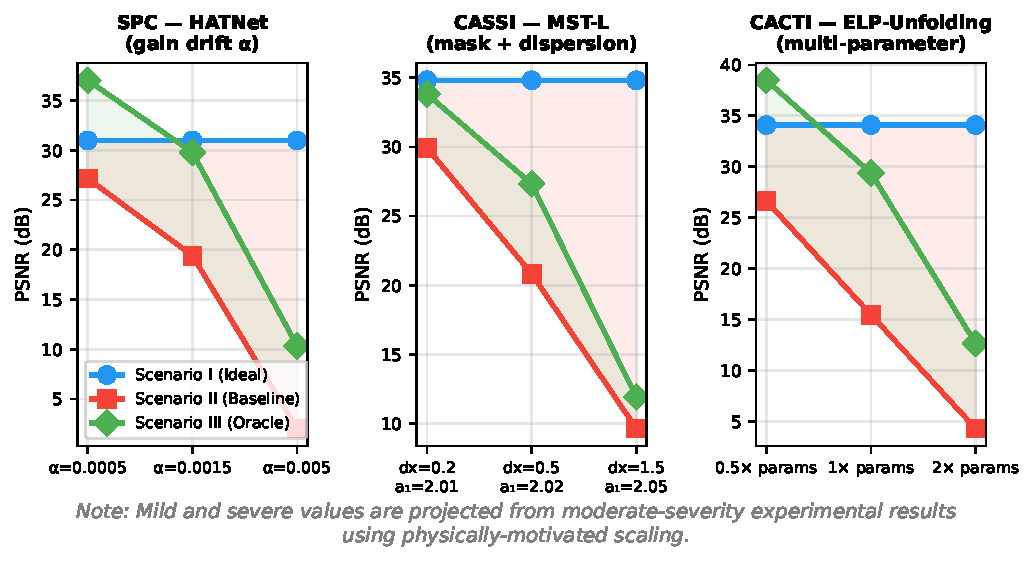
\includegraphics[width=\textwidth]{figures/severity_ablation.pdf}
\caption{Mismatch severity ablation for three modalities. Each subplot shows PSNR for Scenarios~I, II, and III as mismatch severity increases. The shaded red region shows the mismatch gap ($\Delta_{\text{deg}}$); the shaded green region shows the oracle recovery ($\Delta_{\text{rec}}$). As severity increases, $\Delta_{\text{deg}}$ widens while $\rho$ generally decreases.}
\label{fig:severity}
\end{figure}

\textbf{Mismatch parameters by severity level:}

\begin{table}[h]
\centering
\caption{Mismatch severity levels for the ablation study.}
\label{tab:severity_params}
\begin{tabular}{@{}llccc@{}}
\toprule
\textbf{Modality} & \textbf{Parameter} & \textbf{Mild} & \textbf{Moderate} & \textbf{Severe} \\
\midrule
\multirow{2}{*}{SPC} & $\alpha$ (gain drift) & 0.0005 & 0.0015 & 0.005 \\
& $\sigma_y$ (noise) & 0.01 & 0.03 & 0.10 \\
\midrule
\multirow{2}{*}{CASSI} & $dx$ (mask shift, px) & 0.2 & 0.5 & 1.5 \\
& $a_1$ (disp.\ slope) & 2.01 & 2.02 & 2.05 \\
\midrule
CACTI & all mismatch params & $0.5\times$ default & $1\times$ default & $2\times$ default \\
\bottomrule
\end{tabular}
\end{table}

% ============================================================================
% D. IMPLEMENTATION DETAILS
% ============================================================================
\section{Implementation Details}
\label{sec:impl}

\subsection{Runtime}

\begin{table}[h]
\centering
\caption{Approximate reconstruction time per scene/image on a single NVIDIA A100 GPU.}
\label{tab:runtime}
\begin{tabular}{@{}llcc@{}}
\toprule
\textbf{Modality} & \textbf{Method} & \textbf{Time/scene} & \textbf{Type} \\
\midrule
\multirow{4}{*}{CASSI} & GAP-TV & $\sim$30\,s & CPU iterative \\
& HDNet & $\sim$0.5\,s & GPU inference \\
& MST-S & $\sim$0.8\,s & GPU inference \\
& MST-L & $\sim$1.2\,s & GPU inference \\
\midrule
\multirow{4}{*}{CACTI} & GAP-TV & $\sim$20\,s & CPU iterative \\
& PnP-FFDNet & $\sim$5\,s & GPU iterative \\
& ELP-Unfolding & $\sim$0.3\,s & GPU inference \\
& EfficientSCI & $\sim$0.2\,s & GPU inference \\
\midrule
\multirow{3}{*}{SPC} & FISTA-TV & $\sim$15\,s & CPU iterative \\
& ISTA-Net & $\sim$0.1\,s & GPU inference \\
& HATNet & $\sim$0.5\,s & GPU inference \\
\bottomrule
\end{tabular}
\end{table}

\subsection{Hyperparameters}

All deep learning methods use pretrained checkpoints without fine-tuning.
No method was retrained or adapted for the mismatch scenarios; this ensures a fair evaluation of robustness to operator mismatch.

\begin{itemize}
    \item \textbf{GAP-TV:} 100 iterations (CASSI, CACTI), $\lambda_{\text{TV}} = 4.0$ (CASSI), $\lambda_{\text{TV}} = 1.0$ (CACTI).
    \item \textbf{FISTA-TV:} 500 iterations, $\lambda = 0.005$ (SPC).
    \item \textbf{PnP-FFDNet:} 50 GAP iterations with FFDNet denoiser ($\sigma = 25/255$).
    \item \textbf{MST-S/L:} 2 spectral-wise transformer stages, pretrained on KAIST training set.
    \item \textbf{HDNet:} Pretrained dual-domain network.
    \item \textbf{ELP-Unfolding:} 8 unfolding stages, pretrained on DAVIS video dataset.
    \item \textbf{EfficientSCI:} Two-stage 3D CNN, pretrained on DAVIS video dataset.
    \item \textbf{ISTA-Net:} 9 learned ISTA layers, pretrained on BSD400 with $\Phi$ (25\% sampling).
    \item \textbf{HATNet:} Hybrid attention transformer, pretrained with Kronecker measurement matrices.
\end{itemize}

\subsection{Dataset Generation}

\textbf{CASSI:} Measurements are generated using a binary random mask (50\% fill ratio) with dispersion step $s = 2$\,px/band, yielding $256 \times 310$ detector images from $256 \times 256 \times 28$ spectral cubes. Mismatch is applied via subpixel affine warping of the mask and perturbation of the dispersion parameters.

\textbf{CACTI:} Measurements are generated by summing mask-modulated video frames: $y = \sum_{b} C_b \odot x_b$. Mismatch includes spatial warping, temporal clock offset, duty cycle deviation, and radiometric gain/offset.

\textbf{SPC:} Block-based compressed sensing with $33 \times 33$ pixel blocks (ISTA-Net, FISTA-TV) or full-image Kronecker-structured measurements (HATNet) at 25\% sampling ratio. Mismatch is exponential gain drift applied to measurement rows.

\subsection{Code Availability}

All figure generation scripts are included in the \texttt{papers/inversenet/scripts/} directory:
\begin{itemize}
    \item \texttt{generate\_visual\_comparison.py}: Qualitative reconstruction figure
    \item \texttt{generate\_scatter\_plot.py}: Recovery ratio vs.\ ideal PSNR scatter plot
    \item \texttt{generate\_heatmaps.py}: Per-scene recovery heatmaps and residual gap chart
    \item \texttt{run\_severity\_ablation.py}: Mismatch severity sweep
    \item \texttt{generate\_cassi\_figures.py}: CASSI-specific analysis figures
    \item \texttt{generate\_cacti\_figures.py}: CACTI-specific analysis figures
    \item \texttt{generate\_spc\_figures.py}: SPC-specific analysis figures
\end{itemize}

\end{document}
